\chapter{Controllers}\label{ch:controllers}

With the environments defined, it is now necessary to look at the programmable control system of the drones. Indeed, before any manipulation and creation of algorithms, it is important to define all the actions that can be performed by the drones.

This chapter describes the flight controllers of the drones considered and presents the generic control interface, compatible with any model of drone, created for this work.

\section{Drone models}

In this project, two drone models are considered: the simulated drone and the real one.

\subsection{Simulated drone}

The default simulated drone model in AirSim is a Parrot AR Drone 2.0 \cite{wikipedia2021parrotardrone} (Figure \ref{fig:04.parrot.ar.drone.2.0.illustration}).

\begin{figure}[H]
    \centering
    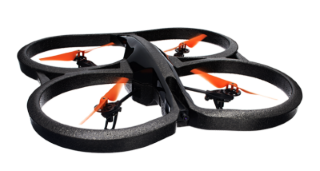
\includegraphics[width=0.4\textwidth]{resources/png/04/parrot-ar-drone-2.0.png}
    \caption{Illustration of the Parrot AR Drone 2.0. \cite{freepng2021parrotardrone}}
    \label{fig:04.parrot.ar.drone.2.0.illustration}
\end{figure}

This drone is a quadcopter equipped with a high-definition front camera and is remotely controlled via Wi-Fi. It is fully programmable and has been designed mainly for experimenting with control algorithms. The main characteristics of this drone are presented in Table \ref{tab:04.parrot.ar.drone.2.0.characteristics}.

\begin{table}[H]
    \centering
    \begin{tabular}{|l|l|p{4cm}|}
        \hline
        \multirow{3}{*}{\textbf{Physical characteristics}} & Weight & $\SI{380}{\gram}$ \\ \cline{2-3}
        & Dimensions (width $\times$ height) & $\SI{45.1}{\centi\meter} \times \SI{45.1}{\centi\meter}$ \\ \cline{2-3}
        & Sensors & Gyroscope, accelerometer, magnetometer, pressure sensor, ultrasound sensor \\ \hline
        \hline
        \multirow{4}{*}{\textbf{Performances}} & Maximum flight distance & $\SI{50}{\meter}$ \\ \cline{2-3}
        & Maximum flight speed & $\SI{5}{\meter\per\second}$ \\ \cline{2-3}
        & Maximum flight time & $\SI{12}{\minute}$ \\ \cline{2-3}
        & Maximum flight height & $\SI{50}{\meter}$ \\ \hline
        \hline
        \multirow{2}{*}{\textbf{Front camera}} & Resolution & HD, 720p, 30 FPS \\ \cline{2-3}
        & Field of view & $\SI{92}{\degree}$ \\ \hline
    \end{tabular}
    \caption{Main characteristics of the Parrot AR Drone 2.0. \cite{wikipedia2021parrotardrone, grosbill2021parrotardrone}}
    \label{tab:04.parrot.ar.drone.2.0.characteristics}
\end{table}

It should be noted that, as the drone is simulated, these characteristics are not all rigorously applied in AirSim. Indeed, it is possible to manually configure the size, the maximum flight speed, the resolution and the field of view of the camera, etc.

\subsection{Real drone}

The real drone model is a Tello EDU \cite{ryzerobotics2021telloedu} (Figure \ref{fig:04.tello.edu.illustration}), manufactured by the Ryze Robotics company and equipped with flight technologies from the DJI company.

\begin{figure}[H]
    \centering
    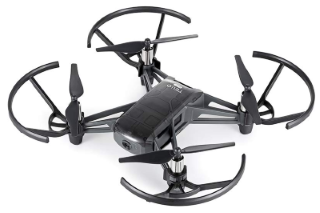
\includegraphics[width=0.4\textwidth]{resources/png/04/tello-edu.png}
    \caption{Illustration of the Tello EDU. \cite{robotadvance2021telloedu}}
    \label{fig:04.tello.edu.illustration}
\end{figure}

This drone is also a quadcopter equipped with a high-definition front camera and is remotely controlled via Wi-Fi. Also being fully programmable, this drone is mainly used to experiment with programmed flight. The main characteristics of this drone are presented in Table \ref{tab:04.tello.edu.characteristics}.

\begin{table}[H]
    \centering
    \begin{tabular}{|l|l|p{4cm}|}
        \hline
        \multirow{3}{*}{\textbf{Physical characteristics}} & Weight & $\SI{87}{\gram}$ \\ \cline{2-3}
        & Dimensions (width $\times$ height) & $\SI{9.8}{\centi\meter} \times \SI{9.2}{\centi\meter}$ \\ \cline{2-3}
        & Sensors & Range finder, barometer, LED \\ \hline
        \hline
        \multirow{4}{*}{\textbf{Performances}} & Maximum flight distance & $\SI{100}{\meter}$ \\ \cline{2-3}
        & Maximum flight speed & $\SI{8}{\meter\per\second}$ \\ \cline{2-3}
        & Maximum flight time & $\SI{13}{\minute}$ \\ \cline{2-3}
        & Maximum flight speed & $\SI{30}{\meter}$ \\ \hline
        \hline
        \multirow{2}{*}{\textbf{Front camera}} & Resolution & HD, 720p, 30 FPS \\ \cline{2-3}
        & Field of view & $\SI{82.6}{\degree}$ \\ \hline
    \end{tabular}
    \caption{Main characteristics of the Tello EDU. \cite{ryzerobotics2021telloedu}}
    \label{tab:04.tello.edu.characteristics}
\end{table}

\subsection{Comparison}

The Parrot AR Drone 2.0 and the Tello EDU are two drones that can be controlled remotely and in a programmable and automatic manner. Although both are designed for experimentation, the AR Drone 2.0 is aimed at a more experienced public, whereas the Tello EDU is aimed at a younger, less experienced public. The latter comes with two mobile applications that allow for fun learning about programming.

Both drones are equipped with a fixed high-definition front camera. Their perception of the environment is therefore essentially limited to what is in front of them. This information is important and must be taken into account because it implies that the drones move sideways or backwards \enquote{blindly}.

The AR Drone 2.0 is larger than the Tello EDU. To have the most accurate simulation possible, the simulated drone has been resized in AirSim to match the size of the Tello EDU. Being sufficiently similar, the other characteristics were left unchanged (including the field of view which, despite a difference of almost \SI{10}{\degree}, has no real impact on the obtained results between simulator and real world).

It should be noted that, as both drones are controlled by Wi-Fi, no data processing operations are embedded and performed directly on the drone; everything is done on the computer. This implies that, for this work, the processing time of the algorithms is not critical since they benefit from the power of a computer. However, it is important to bear in mind that, in most real cases, the algorithms will have to run directly on the drone and therefore be as light and optimized as possible.

\section{Flight controller}

A drone consists of a series of sensors and actuators. The purpose of a flight controller is to bring the drone to a desired state using its actuators based on its current state as perceived by its sensors.

\subsection{Simulated drone}

The drone simulated via AirSim is equipped with a flight controller called \enquote{Simple Flight} \cite{airsim2021simpleflight}. This controller has been designed to make life easier for users. It has its own interface and can be used on both simulated and real models, making it easy to adapt algorithms.

Simple Flight can take as input (state of the drone) angular rates, angular levels, speeds or position. Internally, the controller consists of a series of PID controllers to generate an output signal for the actuators.

\subsection{Real drone}

The Tello EDU is equipped with DJI's control technology and digital image stabilization. Not being explicit about their technologies, it is difficult to say how the controller exactly works.

An important characteristic of this controller is that, although it is very good in general, it is not extremely accurate in terms of distance. For example, when the drone has to move from $\SI{2}{\meter}$ forward, it will move correctly along a straight path (in reality, there is a very small deviation, but completely negligible for short distances) but will travel $\num{2} + \varepsilon$ $\SI{}{\meter}$ where $\varepsilon$ is random noise (the latter is approximately quantified in Section \ref{sec:04.simulated.drone}).

This characteristic has a very important implication for the realization of control algorithms: it is not possible to rely entirely on the drone's controllers to move in a fully autonomous and safe manner. It is not, for example, sufficient to tell the drone to \enquote{move $\SI{10}{\meter}$ forward, turn $\SI{90}{\degree}$ clockwise and move $\SI{2}{\meter}$ forward} because there is no guarantee that the distances will be scrupulously respected, which could lead the drone to hit an obstacle or a wall.

\subsection{Utilization}

This work focuses on the realization of high-level autonomous flight algorithms; the drone and their controllers will therefore be used as is. These controllers are sufficiently powerful to achieve high-level control. Indeed, they allow a correct stabilization and displacement with a few inaccuracies.

However, it is important to keep in mind that the flight controller is a very important part of a drone and that its correct implementation, in order to create a drone, is crucial.

\section{High level control interface}

Although each drone can perform the same main actions (take-off, landing, moving), each has its own control interface, usually designed by the manufacturer. To avoid creating navigation algorithms specific to a particular interface, a new high-level control interface has been implemented. The latter defines general control methods and is an additional layer that can be used on top of the manufacturer's control interface.

\subsection{Architecture}

The architecture of the high-level control interface as well as the controllers designed for each drone are shown in Figure \ref{fig:04.control.interface.architecture}.

\begin{figure}[H]
    \centering
    \begin{tikzpicture}
        \umlclass[type=abstract]{Controller}{}{
            \umlvirt{arm() : void} \\
            \umlvirt{disarm() : void} \\
            \umlvirt{takeoff() : void} \\
            \umlvirt{land() : void} \\
            \umlvirt{move(direction : str, distance : float, speed : int) : void} \\
            \umlvirt{rotate(direction : str, angle : float) : void} \\
            \umlvirt{hover() : void} \\
            \umlvirt{picture() : Image} \\
            manual() : void
        }
        \umlsimpleclass[x=-4, y=-5, fill=blue!20]{AirSimDrone}
        \umlsimpleclass[x=4, y=-5, fill=green!20]{TelloEDU}
        \umlclass[x=-4, y=-8, fill=blue!20]{AirSimDroneNoisy}{}{
            noise(value : float) : float
        }
        \umlimpl[geometry=-|]{Controller}{AirSimDrone}
        \umlimpl[geometry=-|]{Controller}{TelloEDU}
        \umlimpl[geometry=-|]{AirSimDrone}{AirSimDroneNoisy}
    \end{tikzpicture}
    \caption{Architecture of the high-level control interface and controllers of each drone considered in this work.}
    \label{fig:04.control.interface.architecture}
\end{figure}

The high-level control interface (\texttt{Controller}) is an abstract class that must be implemented by each drone used. In this work, a controller was implemented for the simulated drone (\texttt{AirSimDrone}) and another for the real drone (\texttt{TelloEDU}). The simulated drone being too precise in its movements, another controller adding noise on displacements was also created (\texttt{AirSimDroneNoisy}).

The common control commands of the interface are described in Table \ref{tab:04.control.commands.description}.

\begin{table}[H]
    \centering
    \begin{tabular}{|l|p{10cm}|}
        \hline
        \textbf{Command} & \textbf{Description} \\ \hline
        \hline
        \texttt{arm} & Arms the drone. Must be called before any other command. \\ \hline
        \texttt{disarm} & Disarms the drone. Must be called after the last command. \\ \hline
        \texttt{takeoff} & Takes the drone into the air. The altitude depends on the manufacturer flight controller. \\ \hline
        \texttt{land} & Land the drone. \\ \hline
        \texttt{move} & Moves the drone in a chosen direction, a chosen distance at a chosen speed. \\ \hline
        \texttt{rotate} & Turns the drone in a chosen direction at a chosen angle. \\ \hline
        \texttt{hover} & Make the drone stay in place. \\ \hline
        \texttt{picture} & Take a picture. \\ \hline
        \texttt{manual} & Enter the manual control mode of the drone (using the the keyboard of the computer). \\ \hline
    \end{tabular}
    \caption{Description of the high-level control interface commands.}
    \label{tab:04.control.commands.description}
\end{table}

The main advantage of working with a similar interface for the simulated and the real drone is that their use is completely interchangeable. An algorithm that moves the simulated drone can be applied directly to the real drone without requiring any changes to the code. In other words, the high-level control of the drone in the different algorithms is totally agnostic of the drone considered.

In order to demonstrate the use of this interface, a simple test was carried out: a series of pre-defined commands were executed by the simulated and the real drone based on the exact same algorithm, requiring no code modification. A small video of this test is available via the following link: \url{https://youtu.be/1kVLT63IXUE}.

The following sections explained how each control interface has been designed using the manufacturer control interface.

\subsection{Simulated drone}\label{sec:04.simulated.drone}

The AirSim plugin already provides a high-level control interface. This has a large set of commands that are only valid in simulation (\eg{} teleport the drone to a specific position) and is specific to the AirSim simulated drone. In order to have interchangeable commands in the algorithms, the high-level control interface in Figure \ref{fig:04.control.interface.architecture} has been implemented as an additional layer to the AirSim interface (\texttt{AirSimDrone} and \texttt{AirSimDroneNoisy}), using only methods that could be applied to a real drone.

\subsubsection{Noisy version}

As the control of the simulated drone is too perfect (\eg{} when we ask the drone to move $\SI{2}{\meter}$ forward, it will move almost exactly $\SI{2}{\meter}$ forward, which is not really realistic), a noisy version was implemented. The noisy controller (\texttt{AirSimDroneNoisy}) is an additional layer to the simulated drone controller (\texttt{AirSimDrone}). It is responsible for calling the simulated drone's commands by adding a noise $\varepsilon$ to the move and rotate command values such that
\begin{equation}
    \varepsilon \sim \mathcal{N}\rbk{\frac{v}{15}, \frac{v}{50}}
\end{equation}
where $v$ is the initial value sent to the command.

This noise corresponds approximately to the noise on the displacements of the Tello EDU, which was approximated experimentally. For this purpose, several trajectories of fixed length were performed (\eg{} move $\SI{2}{\meter}$ forward). Each time the drone completes a trajectory, its position is noted and the deviation from its objective is calculated (manually). Based on $\num{50}$ samples, a noise model was approximated.

It is clear that $\num{50}$ samples are not sufficient to approximate a faithful model of the noise. However, the chosen model seems realistic enough to be used.

\subsection{Real drone}

When the Tello EDU is switched on, it creates a Wi-Fi network. The drone is controlled by connecting a computer to this network and sending data packets via communication sockets. The contents of the packets are described in the user guide supplied with the Tello EDU \cite{ryzerobotics2020telloeduusermanual}.

The high-level control interface in Figure \ref{fig:04.control.interface.architecture} has been implemented as an additional layer to the Tello EDU interface. This is responsible for initiating sockets and sending corresponding messages when commands are called. An additional socket is reserved to retrieve the video stream.

It should be noted that there is a delay of about $\SI{0.5}{\second}$ between the moment where a command is sent and the moment where the drone executes it but also between the images received from the drone and the reality.
